\section{Data}\label{sec:data}

\subsection{Cross Coupling Catalysts}

%#TODO få sendt dette afsnit i appendix, og få lavet nye data plots osv

The data set of interest consists of 7.054 optimized geometries of compounds being candidate structures in oxidative addition 
catalystic process. The optimized geometries will have a binding energy associated with it, that dictates the net energy 
produced by the oxidative addition of a specific transition metal\cite{Meyer2018}, which is the target of our modelling task. 
The original papers set out to further select 557 catalyst candidates which are within a predefined thermodynamic window, and a 
further selection of candidates based on their pricepoint per mol.\\

The molecular compounds are represented as graph structures of nodes and edges. The nodes constitute atoms, and the edges molecular 
connections between atoms. The representation will further consist of Cartesian coordinates provided in the data set, fixing the 
individual nodes in three dimensional space. This also provides the data set with the possibility of deriving distances between the 
nodes, or the length of edges, which are crucial to the modelling efforts.\\ 

The number of number of nodes in the graphs, range from a minimum of 5, a mean of 52.51, to a maximum of 123 nodes. 
A bar plot of the number of graphs in various buckets of node-counts, can be seen below\ref{num_nodes}.\\

\begin{figure}[H]
\caption{Bar plot of number of nodes per graph}
\centering\label{num_nodes}
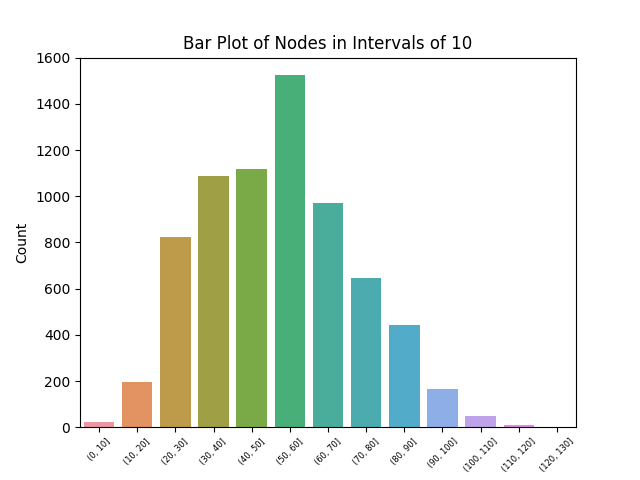
\includegraphics[width=\textwidth]{Images/Data/num_nodes_dataset.png}
\end{figure}

The atom distribution of the graphs a constituted by 13 unique atoms being:
 \begin{itemize}  
 \item H: Hydrogen  
 \item C: Carbon  
 \item N: Nitrogen  
 \item P: Phosphorus  
 \item O: Oxygen  
 \item Cl: Chlorine  
 \item Pd: Palladium  
 \item F: Fluorine  
 \item Au: Gold  
 \item Cu: Copper  
 \item Ag: Silver  
 \item Pt: Platinum  
 \item Ni: Nickel 
 \end{itemize}

The distribution of the above atoms, can be seen in a Pareto graph below\ref{pareto_atoms}. 
The distribution is mainly made up by hydrogen and carbon, those two being 90.6 percent of the atom-representation combined. 
The next highest contributor is nitrogen, only representing 3,4 percent of the atoms. 
The remaining atoms constitute 6 percent of the atom representation in the data set.

\begin{figure}[H]
\caption{Pareto plot of atom distribution in data set}
\centering\label{pareto_atoms}
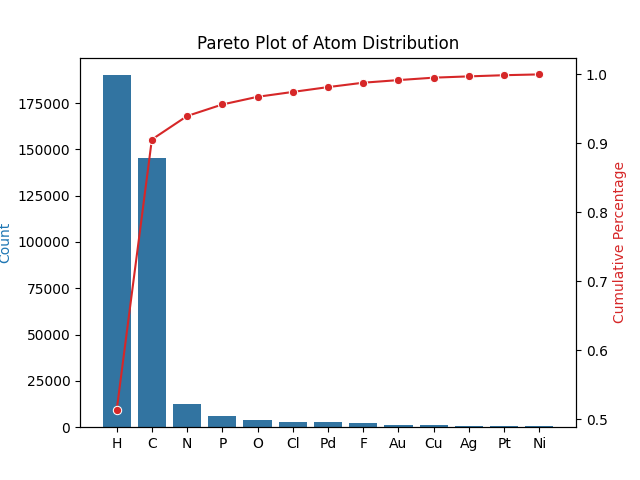
\includegraphics[width=\textwidth]{Images/Data/pareto_atom_distribution.png}
\end{figure}

The additive part of the catalyst process, are selected transition metals, namely: 

\begin{itemize}
  \item Pd: Palladium
  \item Au: Gold
  \item Cu: Copper
  \item Ag: Silver
  \item Pt: Platinum
  \item Ni: Nickel
\end{itemize}

The data set consists of the following distribution of the above transition metals, below can be seen a pareto similar to further above, 
but now show the distribution of transition metals in the data set\ref{addition_atoms}.

\begin{figure}[H]
\caption{Pareto plot of transition metal distribution in data set}
\centering\label{addition_atoms}
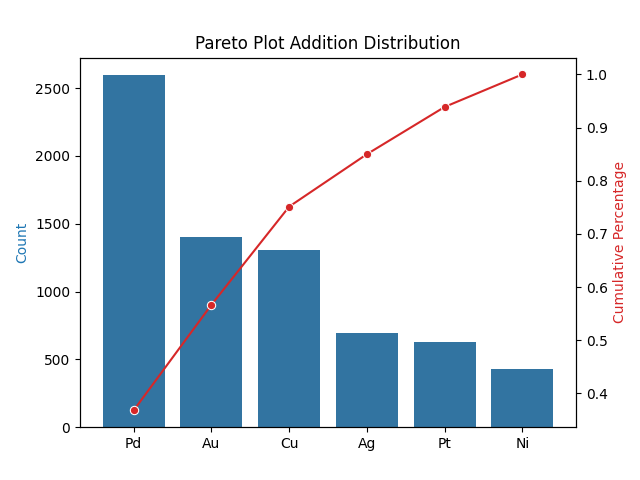
\includegraphics[width=\textwidth]{Images/Data/addition_distribution.png}
\end{figure}

The distribution is mainly comprised of Palladium and Gold, standing for 57 percent of the transition metals in the data set. \\

The catalyst process can be both exothermic and endothermic, represented in either a positive net binding energy as a target, 
or a negative net binding energy as a target for the regression task. The regression targets range from a minimum of -80.82 
being endothermic, to 61.49 being exothermic, where the mean is placed at -18.62. A bar plot with buckets of ten,
 of the distribution of targets can be seen below\ref{binding_energies}.

\begin{figure}[H]
\caption{Bar plot of binding energy distribution in targets}
\centering\label{binding_energies}
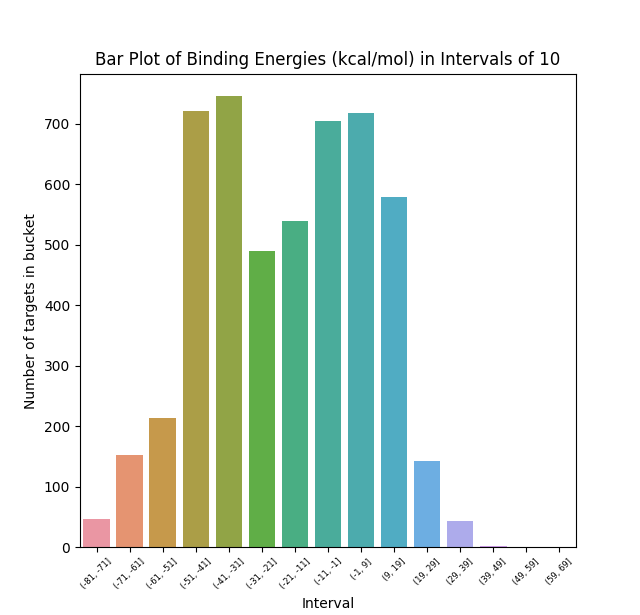
\includegraphics[width=\textwidth]{Images/Data/binding_energies.png}
\end{figure}

The edge-wise distances between nodes, measured in ångstrom, are crucial to the modelling task, since a model-parameter called `r-cut', 
defines a cutoff limit from which edges with a distance lower than the cutoff are defined as neighbours of a given node, and those above 
as non-neighbours. The neighbours goes are allowed a higher model influence, and therefore understanding where to set the cutoff, 
is a crucial hyperparameter. The distances of the full data set is intractable to compute locally, so a subset of 50 randomly chosen 
graphs and their edge-wise distances are plotted as a representation of the full data set\ref{distances}. As we can see in the plot, 
most distances are covered by the interval 0 to 7, at 64 percent, and only 20 percent of distances lie in the interval above 8.5. \\

\begin{figure}[H]
\caption{Pareto plot of Distances between edges from 50 graphs}
\centering\label{distances}
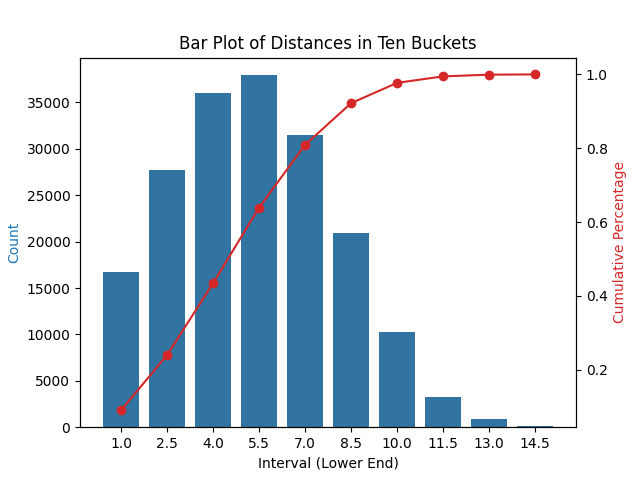
\includegraphics[width=\textwidth]{Images/Data/distances.png}
\end{figure}

In a chemistry context, it is argued that a large portion in the variance in binding energy, can be explained by local interactions 
among atoms\cite{PAINN}. So even though a high degree of information lies beyond cutoff limits of i.e four or five, then information 
might not be crucial to the prediction in energy we are trying to make. \\

The modelling task will take in a given molecular structure, and produce a regression metric, trying to predict the associated 
binding energy from the oxidative addition in the unit kcal/mol. Further more, the regression efforts will be put in an ensemble 
context of a number of structurally similar models, producing a mean and a variance over the predicted regression metric from the 
ensemble.\\

\subsection{Data Privacy- and Quality-issues}

Due to the data sources being publicly available for download, under the creative commons attribution 4.0 license,
 the implementation and storage of the data, has been chosen to support all project activities in the most convenient way. 
 Specifically that mean local and cloud storage, without password protection or encryption of the raw data. \\

The field of chemistry, that this study supports computationally, 
provide research which are used within the life-science industry for drug-discovery among other fields. \\

With this in mind, sourcing of the data set needs to be carefully handled, 
taking into account potential end-user risks of promoting various molecules and processes through research, 
at some point in the process before consumption. The sourcing of the Cross-Coupling data set, is partly transparent. 
The initial data set is comprised of 25.116 graph structures, and was sourced through generating options based on 6 transition metals, 
mentioned above, and 91 ligands. This generation process was made by combining all possible combinations of the six transition metals 
and the 91 ligands, applying a filter for redundant chemical properties to reach the initial 25.116 size data set\cite{Meyer2018}. 
The reduction in data set size to the 7.054, was done by training a model to predict a chemical descriptor value relating to certain 
energy-levels, and then selecting these 7.054 molecules and transition metals based on that. No apparent precaution towards end-user 
complications are mentioned, and should therefore be applied further down stream of the research efforts within this field. 

\newpage

